\documentclass[a4paper]{article}

\usepackage{INTERSPEECH2021}

% Put the lab number of the corresponding exercise
\title{NLU course projects lab 5: NLU}
\name{Nicola Muraro (248449)}

\address{
  University of Trento}
\email{nicola.muraro@studenti.unitn.it}

\begin{document}

\maketitle

\section{Introduction}
In this laboratory, the objective consisted of two tasks: slot filling and intent classification. In the first case, we aim to assign a label to each token within our input sequence to understand the role each token plays within the utterance. In intent classification, on the other hand, we aim to predict a single label for each input sequence, with the goal of extracting the intent of the entire provided input.
To achieve these objectives, we started by using a simple RNN, on which we implemented several techniques to improve performance.
During the second part, we changed the type of architecture, using BERT as the backbone and performing a fine-tuning process on it to align its predictions with our tasks.


\section{Implementation details}
For the first part of the assignment, starting from the architecture provided in the lab, I simply added the bidirectionality to the LSTM component by using the appropriate parameter in the PyTorch function.
Consequently, the output dimension of this component is doubled, as we now have the concatenated outputs of the forward and reverse processes. To ensure compatibility with the network layer responsible for slot prediction, I adjusted its input size by doubling it.
The next modification involved adding dropout to the architecture.
This technique can be applied in various part of the code: after the utterance embedding, before the two prediction heads, or in both places. To determine the optimal position for this technique, I tested all three scenarios separately, allowing me to draw an empirical conclusion.
\newline

In the second part of the assignment, we adopted a different approach to the problem. Starting with BERT, a pretrained language understanding model based on transformers, we performed fine-tuning to adapt the model to our tasks.
This kind of implementation was detailed in the following paper \cite{BERT}. Specifically, the network I designed consists of BERT-base, a dropout layer, and two projection heads (one for each task).
First, the utterance was tokenized using a tokenizer specific to BERT: the BertTokenizer.
Additionally, BERT requires all input utterances to have the same length. Consequently, I added padding to the utterances and slots to ensure uniform length, making them comparable for metric computation and performance evaluation of the created model.
Then, when using the model, the utterance (already tokenized and padded) is passed as input to BERT, which generates an embedding for the provided input. This hidden state is passed through a dropout layer and used as input for both projection heads. The first token in the sequence is utilized by one prediction head to predict the intent, while the remaining tokens are fed into the other prediction head to perform slot filling.

\section{Results}
As in the previous assignment, I used the validation set to adjust the hyperparameters, ignoring their impact on the test set. This approach allows the test set to be evaluated only at the end, providing more reliable performance metrics for the model.

For all the results reported below, I used the Adam optimizer with a learning rate of \(lr = 0.0001\). Additionally, the batch sizes for the train and test sets remained unchanged at \(64\) and \(128\), respectively.

For the first part of the assignment, adding both bidirectionality and dropout layers improved the proposed model’s performance, as shown in Table \ref{tab:results1}. 
Figure \ref{fig:fig1} also provides a visualization of the model's training dynamics. From there we can observe that the model behaves well, with a clear decreasing trend in the loss function on both sets of data.
Specifically, I empirically found that applying dropout both after the utterance embedding and before the two prediction heads yielded the best results.
The configuration used for this part was: \(emb \textunderscore size=300, hid \textunderscore size=300\).
For each test, \(5\) runs were performed, and the resulting values were averaged.


\begin{table}[h]
  \centering
  \begin{tabular}{|c|c|c|}
    \hline
    \textbf{Model} & \textbf{Slot F1} & \textbf{Intent Acc} \\
    \hline
    IAS bidir.&  0.935 +- 0.002 & 0.940 +- 0.004 \\
    IAS bidir. + dropout & 0.940 +- 0.002 & 0.953 +- 0.005 \\
    \hline
  \end{tabular}
  \caption{Slot filling and intent performance for the first part of the assignment. The values shown are obtained by an average of 5 runs on the test set.}
  \label{tab:results1}

\end{table}

\begin{figure}[h]
  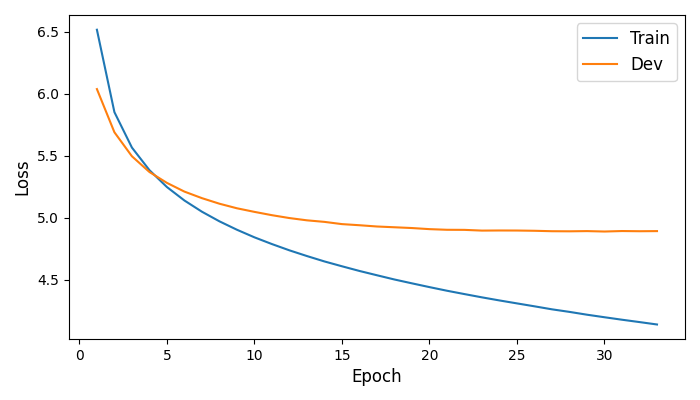
\includegraphics[width=\linewidth]{./images/plot_1_loss.png}
  \caption{Trainig loss for the best model of the first part}
  \label{fig:fig1}
\end{figure}

In the second part, the input size for the two prediction heads had to match the dimension of BERT’s last hidden state. Due to this fact, both were set to 768.
The loss also in this case was a weighted average of the loss for intents and slots. I empirically determined that the best combination was: \(combined \textunderscore loss = loss \textunderscore intent * 0.1 + loss \textunderscore slot * 0.9\).
The performance of this model was evaluated over a single run because the training time for this type of architecture is significantly higher compared to the first one. The results are shown in Table \ref{tab:results2}, while Figure \ref{fig:fig2} illustrates the training dynamics of the model.
As we can see, in the beginning of the train the loss is very high, but after a few epochs it starts to decrease rapidly. This is probably due to the fact that the backbone needs some time to adapt to the new tasks, and then it starts to perform well.

From both tables, we can observe that training a model from scratch achieved slightly better performance than fine-tuning BERT on the slot filling task. Instead, on the intent classification task, the second model is slightly better. 
Still, in both cases the results obtained are very good for both of this tasks.

\begin{table}[h]
  \centering
  \begin{tabular}{|c|c|c|}
    \hline
    \textbf{Model} & \textbf{Slot F1} & \textbf{Intent Acc} \\
    \hline
    BERT finetuned& 0.927 & 0.967 \\
    \hline
  \end{tabular}
  \caption{Slot filling and intent performance for the second part of the assignment. The values shown are obtained in a single run on the test set.}
  \label{tab:results2}
\end{table}

\begin{figure}[h]
  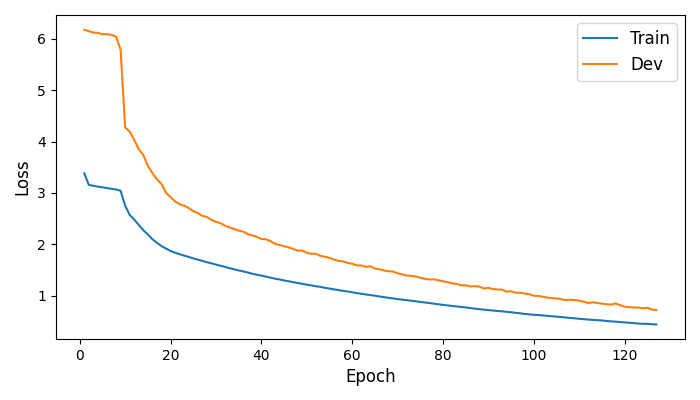
\includegraphics[width=\linewidth]{./images/plot_2_loss.png}
  \caption{Trainig loss for the best model of the second part}
  \label{fig:fig2}
\end{figure}


\bibliographystyle{IEEEtran}

\bibliography{mybib}


\end{document}
